\documentclass[12pt,a4paper]{article}

\usepackage[utf8]{inputenc}
\usepackage{ctex}
\usepackage{amsmath}
\usepackage{graphicx}
\usepackage{float}
\usepackage{booktabs}
\usepackage{geometry}
\usepackage{tikz}
\usepackage{array}

\usetikzlibrary{arrows,positioning,shapes.geometric,calc}

\geometry{margin=0.8in}

\begin{document}

\section*{STAEformer 模型架构}

\vspace{1cm}

\subsection*{1. 整体架构}

\begin{figure}[H]
	\centering
	\begin{tikzpicture}[
			>=stealth,
			node distance=1.5cm and 2cm,
			block/.style={rectangle, draw, fill=blue!20, minimum width=3cm, minimum height=1cm, align=center, font=\small},
			arrow/.style={->, thick}
		]

		\node[block, fill=green!30] (input) {$X$ \\ $(B, 12, 207, 3)$ \\ 原始输入};
		\node[block, right=of input] (proj) {Input \\ Projection};
		\node[block, fill=yellow!30, right=of proj] (embed) {时空自适应 \\ 嵌入融合};
		\node[block, fill=yellow!40, right=of embed] (temporal) {Temporal \\ Attention};
		\node[block, fill=orange!40, right=of temporal] (spatial) {Spatial \\ Attention};
		\node[block, fill=purple!30, right=of spatial] (ff) {Feed \\ Forward};
		\node[block, fill=red!30, right=of ff] (output) {Mixed \\ Projection};
		\node[block, fill=gray!30, right=of output] (result) {$\hat{Y}$ \\ $(B, 12, 207, 1)$};

		\draw[arrow] (input) -> (proj);
		\draw[arrow] (proj) -> (embed);
		\draw[arrow] (embed) -> (temporal);
		\draw[arrow] (temporal) -> (spatial);
		\draw[arrow] (spatial) -> (ff);
		\draw[arrow] (ff) -> (output);
		\draw[arrow] (output) -> (result);

	\end{tikzpicture}
	\caption{整体架构}
\end{figure}

\vspace{1cm}

\subsection*{2. 时空自适应嵌入}

\begin{figure}[H]
	\centering
	\begin{tikzpicture}[
			>=stealth,
			node distance=0.8cm and 1cm,
			tensor/.style={rectangle, draw, fill=blue!20, minimum width=2cm, minimum height=1.5cm, align=center},
			small/.style={rectangle, draw, fill=#1!20, minimum width=2cm, minimum height=0.6cm, font=\small}
		]

		\node[tensor] (T) {$T_{in}=12$};
		\node[tensor, right=of T] (N) {$N=207$};
		\node[tensor, right=of N] (D) {$D_{adp}=80$};

		\node[below=1cm of T, font=\small] {时间步};
		\node[below=1cm of N, font=\small] {节点数};
		\node[below=1cm of D, font=\small] {嵌入维度};

		\node[right=2cm of D, tensor, fill=purple!30] (E) {$E_{adp}$};
		\node[right=0.5cm of E, font=\small] {$= 198,720$ 参数};

	\end{tikzpicture}
	\caption{自适应嵌入矩阵}
\end{figure}

\begin{figure}[H]
	\centering
	\begin{tabular}{m{2cm} m{4cm} m{2cm}}
		\hline
		嵌入类型        & 维度            & 说明                                                        \\
		\hline
		Input Embed & 24维           & 线性投影 $W_{proj}: \mathbb{R}^3 \rightarrow \mathbb{R}^{24}$ \\
		ToD Embed   & 24维           & 时间 embedding, 288步/天                                      \\
		DoW Embed   & 24维           & 星期 embedding, 7天                                          \\
		Adaptive    & 80维           & 可学习参数 $E_{adp} \in \mathbb{R}^{12 \times 207 \times 80}$  \\
		\hline
		\textbf{总计} & \textbf{152维} &                                                           \\
		\hline
	\end{tabular}
	\caption{嵌入融合详情}
\end{figure}

\vspace{1cm}

\subsection*{3. 多头自注意力}

\begin{figure}[H]
	\centering
	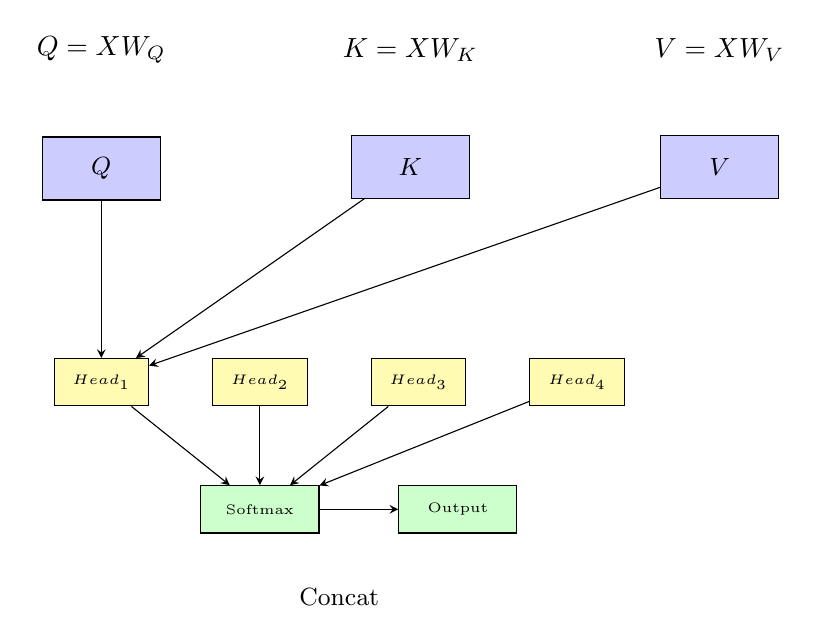
\begin{tikzpicture}[
			>=stealth,
			node distance=0.5cm and 1cm,
			qkv/.style={rectangle, draw, fill=blue!20, minimum width=1.5cm, minimum height=0.8cm, font=\small},
			head/.style={rectangle, draw, fill=yellow!30, minimum width=1.2cm, minimum height=0.6cm, font=\tiny},
			op/.style={rectangle, draw, fill=green!20, minimum width=1.5cm, minimum height=0.6cm, font=\tiny}
		]

		\node (Q) {$Q = XW_Q$};
		\node[right=2cm of Q] (K) {$K = XW_K$};
		\node[right=2cm of K] (V) {$V = XW_V$};

		\node[below=0.8cm of Q, qkv] (Qb) {$Q$};
		\node[below=0.8cm of K, qkv] (Kb) {$K$};
		\node[below=0.8cm of V, qkv] (Vb) {$V$};

		\node[below=2cm of Qb, head] (h1) {$Head_1$};
		\node[right=0.8cm of h1, head] (h2) {$Head_2$};
		\node[right=0.8cm of h2, head] (h3) {$Head_3$};
		\node[right=0.8cm of h3, head] (h4) {$Head_4$};

		\node[below=1cm of h2, op] (score) {Softmax};
		\node[right=1cm of score, op] (out) {Output};

		\draw[->] (Qb) -- (h1);
		\draw[->] (Kb) -- (h1);
		\draw[->] (Vb) -- (h1);

		\draw[->] (h1) -- (score);
		\draw[->] (h2) -- (score);
		\draw[->] (h3) -- (score);
		\draw[->] (h4) -- (score);

		\draw[->] (score) -- (out);

		\node at ($(h1)!0.5!(h4)$) [below=2.5cm, font=\small] {Concat};

	\end{tikzpicture}
	\caption{多头注意力 (4 heads)}
\end{figure}

公式:
$$Attention(Q_i, K_i, V_i) = softmax\left(\frac{Q_i K_i^T}{\sqrt{d_k}}\right) V_i$$

\vspace{1cm}

\subsection*{4. 时空交替Transformer层}

\begin{figure}[H]
	\centering
	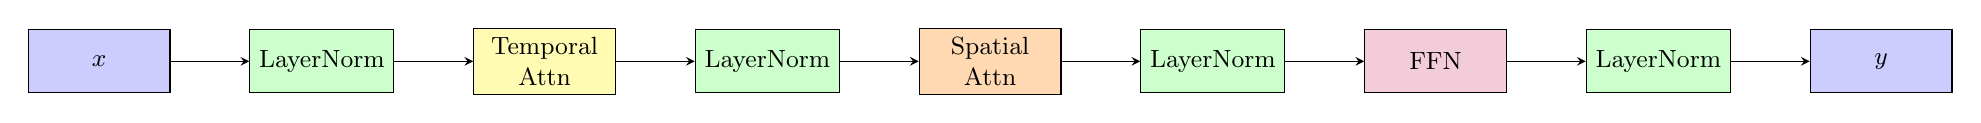
\begin{tikzpicture}[
			>=stealth,
			node distance=0.3cm and 1cm,
			layer/.style={rectangle, draw, fill=blue!20, minimum width=1.8cm, minimum height=0.8cm, font=\small, align=center}
		]

		\node[layer] (x) {$x$};
		\node[layer, fill=green!20, right=of x] (ln1) {LayerNorm};
		\node[layer, fill=yellow!30, right=of ln1] (ta) {Temporal\\Attn};
		\node[layer, fill=green!20, right=of ta] (ln2) {LayerNorm};
		\node[layer, fill=orange!30, right=of ln2] (sa) {Spatial\\Attn};
		\node[layer, fill=green!20, right=of sa] (ln3) {LayerNorm};
		\node[layer, fill=purple!20, right=of ln3] (ff) {FFN};
		\node[layer, fill=green!20, right=of ff] (ln4) {LayerNorm};
		\node[layer, right=of ln4] (y) {$y$};

		\draw[->] (x) -> (ln1);
		\draw[->] (ln1) -> (ta);
		\draw[->] (ta) -> (ln2);
		\draw[->] (ln2) -> (sa);
		\draw[->] (sa) -> (ln3);
		\draw[->] (ln3) -> (ff);
		\draw[->] (ff) -> (ln4);
		\draw[->] (ln4) -> (y);

	\end{tikzpicture}
	\caption{STAE Layer ($\times 3$)}
\end{figure}

\vspace{1cm}

\subsection*{5. Mixed Projection 输出}

\begin{figure}[H]
	\centering
	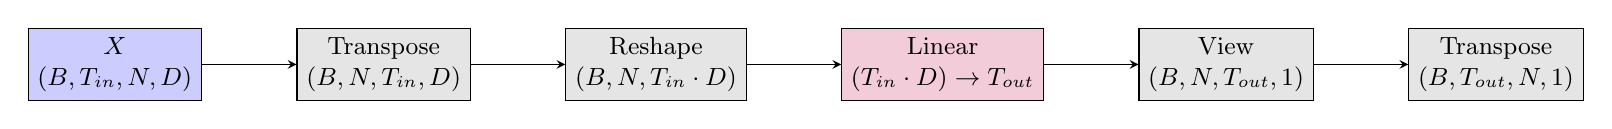
\begin{tikzpicture}[
			>=stealth,
			node distance=0.5cm and 1.2cm,
			box/.style={rectangle, draw, fill=#1!20, minimum width=2.2cm, minimum height=0.9cm, font=\small, align=center}
		]

		\node[box=blue] (x1) {$X$ \\ $(B, T_{in}, N, D)$};
		\node[right=of x1, box=gray] (t) {Transpose \\ $(B,N,T_{in},D)$};
		\node[right=of t, box=gray] (r) {Reshape \\ $(B,N,T_{in} \cdot D)$};
		\node[right=of r, box=purple] (l) {Linear \\ $(T_{in} \cdot D) \rightarrow T_{out}$};
		\node[right=of l, box=gray] (v) {View \\ $(B,N,T_{out},1)$};
		\node[right=of v, box=gray] (t2) {Transpose \\ $(B,T_{out},N,1)$};

		\draw[->] (x1) -> (t);
		\draw[->] (t) -> (r);
		\draw[->] (r) -> (l);
		\draw[->] (l) -> (v);
		\draw[->] (v) -> (t2);

	\end{tikzpicture}
	\caption{输出映射}
\end{figure}

\vspace{1cm}

\subsection*{6. 模型配置参数表}

\begin{table}[H]
	\centering
	\begin{tabular}{|l|r|l|}
		\hline
		参数                       & 默认值 & 说明            \\
		\hline
		num\_nodes               & 207 & 节点数           \\
		in\_steps                & 12  & 输入时间步         \\
		out\_steps               & 12  & 输出时间步         \\
		steps\_per\_day          & 288 & 每日步数          \\
		input\_dim               & 3   & 输入维度          \\
		output\_dim              & 1   & 输出维度          \\
		input\_embedding\_dim    & 24  & 输入嵌入          \\
		tod\_embedding\_dim      & 24  & 时间嵌入          \\
		dow\_embedding\_dim      & 24  & 星期嵌入          \\
		adaptive\_embedding\_dim & 80  & 自适应嵌入         \\
		feed\_forward\_dim       & 256 & FFN维度         \\
		num\_heads               & 4   & 注意力头数         \\
		num\_layers              & 3   & Transformer层数 \\
		model\_dim               & 152 & 模型总维度         \\
		\hline
	\end{tabular}
\end{table}

\end{document}